\chapter{Teaching a robot to support child learning}\label{chap:education}
\graphicspath{{images/education/}}

\begin{framed}
	\textbf{Key points:}
	
	\begin{itemize}
		\item An experiment was designed to test \gls{sparc} in the wild in a learning application in a school.
		\item Between participant study involving 70 children compared 3 conditions: passive robot, supervised robot and autonomous robot.
		\item .
		\item .
		\item .
	\end{itemize}
\end{framed}

Parts of the work presented in this chapter have been published verbatim in \cite{senft2017toward} \footnote{Note about technical contribution in this chapter: the author reimplemented every part of the system manually in Qt.}. The final publication is available from AAAI via \url{https://aaai.org/ocs/index.php/FSS/FSS17/paper/view/16011}.

\newpage
\section{Motivation}

Chapters \ref{chap:woz} and \ref{chap:control} tested \gls{sparc} in interactions between robots or in a virtual world but not for human-robot interactions as it was developed for. As such a new study had to evaluate the application of \gls{sparc} to teach a robot an interactive behaviour in a real human-robot interaction. It has been decided to focus on robots in education to teach a food-web to children as it provides a constraints while rich and complex environment for the interaction. The scenario and the code is based on \cite{lemaignan2017free} but has been adapted to provide a robot controller and task goal for the children.

\section{Setup of the study}

Similarly to the study presented in Chapter \ref{chap:woz}, this study is based on the Sandtray paradigm \citep{baxter2012touchscreen}: a child interacts with a robot through a large touchscreen located between them. Additionally, a teacher can use a tablet to control the robot in one of the conditions (cf. Figures \ref{fig:education_setup} and Figure \ref{fig:setup} used to frame this research).

\begin{figure}[ht]
	\centering
	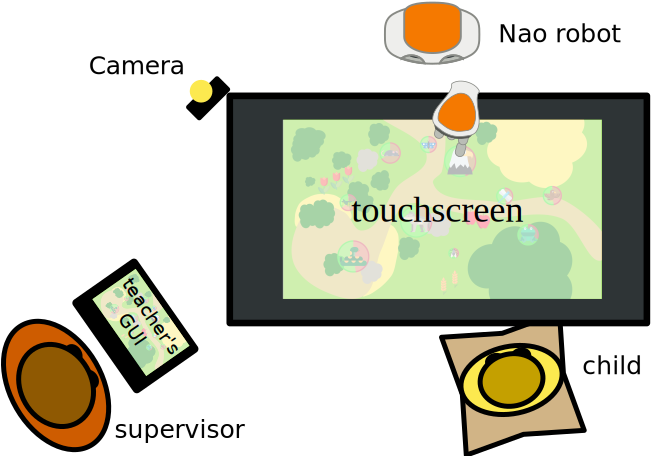
\includegraphics[width=.5\textwidth]{setup.jpg}
	\caption{Setup used in the study: a child interacts with the robot tutor, with a large touchscreen sitting between them displaying the learning activity; a human teacher provides guidance to the robot through a tablet and monitors the robot learning.}
	\label{fig:education_setup}
\end{figure}



\subsection{Food chain game}
To teach children a food web, they interacted with a game presented 10 animals and three types of plants. Animals have energy decreasing over time and they have to eat to stay healthy. Animals are immobile unless the child or the robot move them and eat or be eaten when entering in contact with another animal or a plant. Children have to feed animals by moving them to their food, and by feeding them can learn what food each animal eats. Figure \ref{fig:education_game} presents an example of the game where after some time each animal has lost some energy

\begin{figure}[ht]
	\centering
		\includegraphics[width=1\textwidth]{game.png}
		\captionsetup{width=.9\linewidth}
		\caption{Example of the game. Animals have energy in red and have to eat plants of other animals to survive.}
		\label{fig:education_game}
\end{figure}

\subsection{Robot behaviour}
 
During the game, the robot can execute actions to provide hints and support to the child. The robot has access to five types of actions:
\begin{itemize}
	\item Movements: moving any animal to, toward or away from other item (animal or plant) - the robot points to an animal and moves it on the game while describing its action (e.g. "The eagle needs help getting close to the mouse").
	\item Drawing attention: the robot points an item and says a reminder to the child (e.g. "Don't forget the frog").
	\item Reminding rules: the robot says one of 5 sentences on the game (e.g. "Move the animals to feed them" or "Don't feed animals with a lot of energy").
	\item Congratulation: the robot provides congratulations (e.g. "Well done").
	\item Encouragements: the robot provides encouragement (e.g. "You can do it").
\end{itemize}

For each utterance joining an action, multiple versions are available, and a random one not used recently is selected. Considering all the possible combination, the total number of  actions adds up 655.

These actions represent different level of support, from general motivation and informations sentences to information about which animals the child should focus on or direct information about what animals eat. This should cover a large range of supportive feedback provided for such an application. 

\subsection{Wizard of Oz application}

To allow the interaction between the teacher and the robot, a \gls{gui} has been developed representing the current state of the game exactly as the child sees it on the touchscreen \ref{fig:education_gui}. Buttons for the actions (excluding movements) allow the teacher to select which action the want the robot to execute. To provide additional features for the algorithms and precise which action the teacher is executed (on which animal should the robot draw the attention), the teacher can select animals or plant and provide them to the other components. For example, if the teacher highlights the frog and then press the "Draw attention" button, the actions \textit{drawing attention to the frog} will be executed by the robot.

For the movements, the teacher can drag the the image of the animals, creating a \textit{shadow} and the release of this shadow triggers the start of the motion. Depending the animal moved and the other items highlighted, the corresponding action will be inferred and sent to the robot. This gives access to the teacher to the full 655 actions without requiring as many buttons.

\begin{figure}[ht]
	\centering
	\includegraphics[width=1\textwidth]{gui.png}
	\captionsetup{width=.9\linewidth}
	\caption{\gls{gui} used by the teacher to control the robot and respond to its suggestions. The game presents the same state as in Figure \ref{fig:education_game}, and he robot proposes to move the frog close to the fly (text bubble, arrow, moving the \textit{shadow} of the frog and highlight of the frog and the fly).}
	\label{fig:education_gui}
\end{figure}

Additionally, the \gls{gui} is used by the teacher to respond to the propositions of the robot. Following the proposition of an action, a bubble describing the action will appear on top of the \gls{gui} and the corresponding item will be highlighted and if the action is a motion, an arrow will show the proposed motion. The teacher can react to the proposed action by pressing the "Do it", "Skip", "Cancel" or "Remove" buttons or let the action be executed. The action will be automatically executed after 2 seconds, during which the bubble will become greener to represent the passive acceptance of the action. The "Do it" button executes the action straight-away, the "Skip" button informs the algorithm that it should wait rather than doing the action, the "Cancel" button assigns a negative reward to this action in that case and finally, the "Remove" button looks for the closest previous instantiation of action in memory and removes it, preventing it to be executed later.

\subsection{Algorithm}

To learn a appropriate action policy, the algorithm has to map an action (or no action) to each possible state. The state used in this study represents the state of the game in a 210 dimensional vector, with value from 0 to 1. The dimensions include: distance between items, items' energy, time since events (child and robot touching each animal, robot's actions, interaction events: feeding an animal, death of animal...), progression in the game sessions and child face direction (toward the robot, the screen or away).

The actions and the state dimensions have been selected to be generic to many teaching task involving movable items: each item can have a value assigned to it (here energy, but this could be changed in other scenario), and some movable items (here animals) can be move toward or away from other items. Using these generic actions and this state definition, this implementation could be easily re-purposed to another teaching task.

The algorithm used for the learning is an adaptation of the one presented in \cite{senft2017toward}. It is an instance based algorithm similar to the nearest-neighbours algorithm \cite{cover1967nearest}. However, two differences are notable compared to the initial algorithm. Firstly, instead of being defined on the full state space, instances are defined on a sliced version of the state. The intuition is that states needed to cover complex action policy require large number of dimensions, however for a single action, large parts of the state are irrelevant: for example if a robot needs to pick-up a cup, the colour of the cup does not impact the optimal motion. For this implementation, when selecting actions, the teacher can highlight features of the environment which will \textit{activate} specific dimensions of the state space that are used to store the instance in memory. All \textit{non-activated} dimensions are left as wild-card. Then when comparing the current state to the saved instances, the distance is only computed on the \textit{activated} dimensions of the comparing instance. The second difference is that each instance saved has a reward assigned to it, if the teacher selected the action, a reward of $+1$ is assigned, and if the teacher cancelled the action (following an incorrect suggestion from the algorithm) a reward of $-1$ is assigned. When selecting an action, the algorithm looks through all the actions it have been using and for each action selects the closest instance and compute the expected reward as a multiplication of the distance with the reward assigned. Then the algorithm selects the action with the highest expected reward and proposes it if the value is higher than an adaptive threshold. 

The algorithm runs at 2Hz while we would expect actions to be selected every 5 to 20 seconds, so unlike most of the discrete cases of action selections, in most of the steps, no actions are required. To handle this difference of timescale, a waiting action have been added (through the ``skip button'') and an adaptive threshold only proposes actions with an expected reward higher than the threshold. Selecting an action can reduce the threshold, and cancelling or skipping an action can increase it. This adapts the rate of action propositions to the desires of the teacher. Another mechanism filters propositions from the algorithm not to transfer them to the teacher when an action is already proposed to the supervisor or the robot is acting and also rewards negatively impossible actions (such as moving dead animals).

\section{Methodology}

\subsection{Study design}

Sixty children aged 8 to 10 participated in the study (age: \textit{M}=8.9, \textit{SD}=0.83; 11F/15M).  Children were first introduced to the robot and the aim of the interaction, then had a first pre-test to evaluate their initial knowledge. Before starting the teaching game, children have to complete a tutorial where they are introduced to the mechanics of the game: animals have life and have to eat to survive and children can move animals to make them interact with other animals or plants. After this short tutorial, they have to complete two sessions of the game where the robot can provide feedback and advices depending which conditions they are in. After these initial sessions of the game they have to complete a mid-test before playing another 2 sessions of the game and a last post-test before concluding the study. 

\begin{figure}[h]
	\includegraphics[width=.9\linewidth]{graph.png}
	\centering
	\caption{Methodology used for the study.}
	\label{fig:method}
\end{figure}

In all the conditions, the robot's behaviour during the introduction, tests, tutorial and conclusion is identical. The only change of behaviour happens during the games sessions. Figure \ref{fig:game} shows an example of the game screen. The child can move 10 animals across the game field and can have them interact with other animals or plants. Animals lose energy over time and by interacting with their food the can regain some. Animals that are eaten lose a chunk of their life. The goal for the children is to keep animals alive as long as possible by feeding them and they earn stars representing how healthy their animals have been during the session. The game stops when 3 or more animals run out of energy and each game session lasted 1.6 minutes in average.

\subsection{Hypotheses}

\subsection{Metrics}
\subsubsection{Learning Evaluation}
During the pre-test, the experimenter demonstrate how to connect animals by drawing an arrow from the frog to the fly, and they removing the arrow by pressing the \textit{X} button. Then, children are asked to connect as many animals as possible. Figure \ref{fig:test} shows two examples of test, without or with all correct connections. When they think they are done, they can press the continue button, showing a screen asking confirmation to quit the test or give the opportunity to keep connecting animals. Additionally, the robot inform the child if not all the animals are connected to their food or that animal can eat many types of food if no more than one animal has been connected to two items. They are in total 25 different correct connections and 95 possible incorrect ones. As the child can connect as many arrows as desired, the performance is defined as the number of correct arrows above chance for the total number of connected arrows on the test divided by the maximum achievable performance to reach a score with a ceiling at 1.

\begin{figure*}[ht]
	\centering
	\begin{subfigure}[t]{0.5\textwidth}
		\centering
		\includegraphics[width=0.95\textwidth]{empty_graph.png}
		\captionsetup{width=.95\linewidth}
		\caption{Empty screen that children face at each test. Red dots behind animals represent that they are not been connected to any food.}
		\end{subfigure}%
		~ 
		\begin{subfigure}[t]{0.5\textwidth}
			\centering
			\includegraphics[width=0.95\textwidth]{full_graph.png}
			\captionsetup{width=.95\linewidth}
			\caption{Fully connected test with all the correct connections.}
			\end{subfigure}
			\caption{Test screen to evaluate children's knowledge, empty starting screen (a) and fully connected and correct test (b).}
			\label{fig:test}
			\end{figure*}
\section{Results}

\section{Discussion}

\section{Summary}

